\item Consider a uniform spherical charge distribution of radius \( R_1 \) centred at the origin \( O \). In this distribution, a spherical cavity of radius \( R_2 \), centred at \( P \) with distance \( OP = a = R_1 - R_2 \) (see figure) is made. If the electric field inside the cavity at position \( \vec{r} \) is \( \vec{E}(\vec{r}) \), then the correct statement(s) is(are)
\begin{center}
    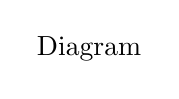
\begin{tikzpicture}
    \node {Diagram};
    \end{tikzpicture}
\end{center}
    \begin{tasks}(1)
        \task \( \vec{E} \) is uniform, its magnitude is independent of \( R_2 \) but its direction depends on \( \vec{r} \)
        \task \( \vec{E} \) is uniform, its magnitude depends on \( R_2 \) and its direction depends on \( \vec{r} \)
        \task \( \vec{E} \) is uniform, its magnitude is independent of \( a \) but its direction depends on \( \vec{r} \)
        \task \( \vec{E} \) is uniform and both its magnitude and direction depend on \( \vec{r} \)
    \end{tasks}

